\chapter{State of Artificial Intelligence }
%longtable for review

\section{Introduction}
%In this chapter, we delve into the foundation of our AI assistance, the large language model, which serves as the powerful engine of our system. Meanwhile, understanding the current state of artificial intelligence is imperative to harnessing its capabilities effectively. Therefore, we explore the landscape of artificial intelligence in its current form to contextualize the development of our AI assistance.
In this chapter, we discuss the foundation of our AI assistance, the large language model, which is like the powerful engine of our system. Meanwhile, it is very important to understand the current state of artificial intelligence in order to use its capabilities properly. Therefore, we explore the landscape of artificial intelligence in its current form to contextualize the development of our AI assistance. 
\section{Large language model (LLM)}
\subsection{Definition}
At its core, a large language model is a type of computer program that can understand and create human language using neural networks. The main job of a language model is to figure out the chances of a word coming next in a sentence. For instance, in the sentence "The sky is ......" the most common answer would be "blue". The model can guess the next word in a sentence by looking at a big collection of text. Basically, it learns to recognize patterns in the words. You get a pre-trained language model from this process
%At its core, a large language model is a type of machine learning model that can understand and generate human language via deep neural networks. The main job of a language model is to calculate the probability of a word following a given input in a sentence: for example, “The sky is .......” with the most likely answer being “blue”. The model is able to predict the next word in a sentence after being given a large text dataset (or corpus). Basically, it learns to recognize different patterns in the words. From this process, you get a pre-trained language model.
\vskip 0.5cm
The following \textbf{Figure \ref{fig:artificial-intelligence}} \cite{w9} illustrates the layers within the field of Artificial Intelligence.
\begin{figure}[H]
    \label{fig:artificial-intelligence}
    \centering
    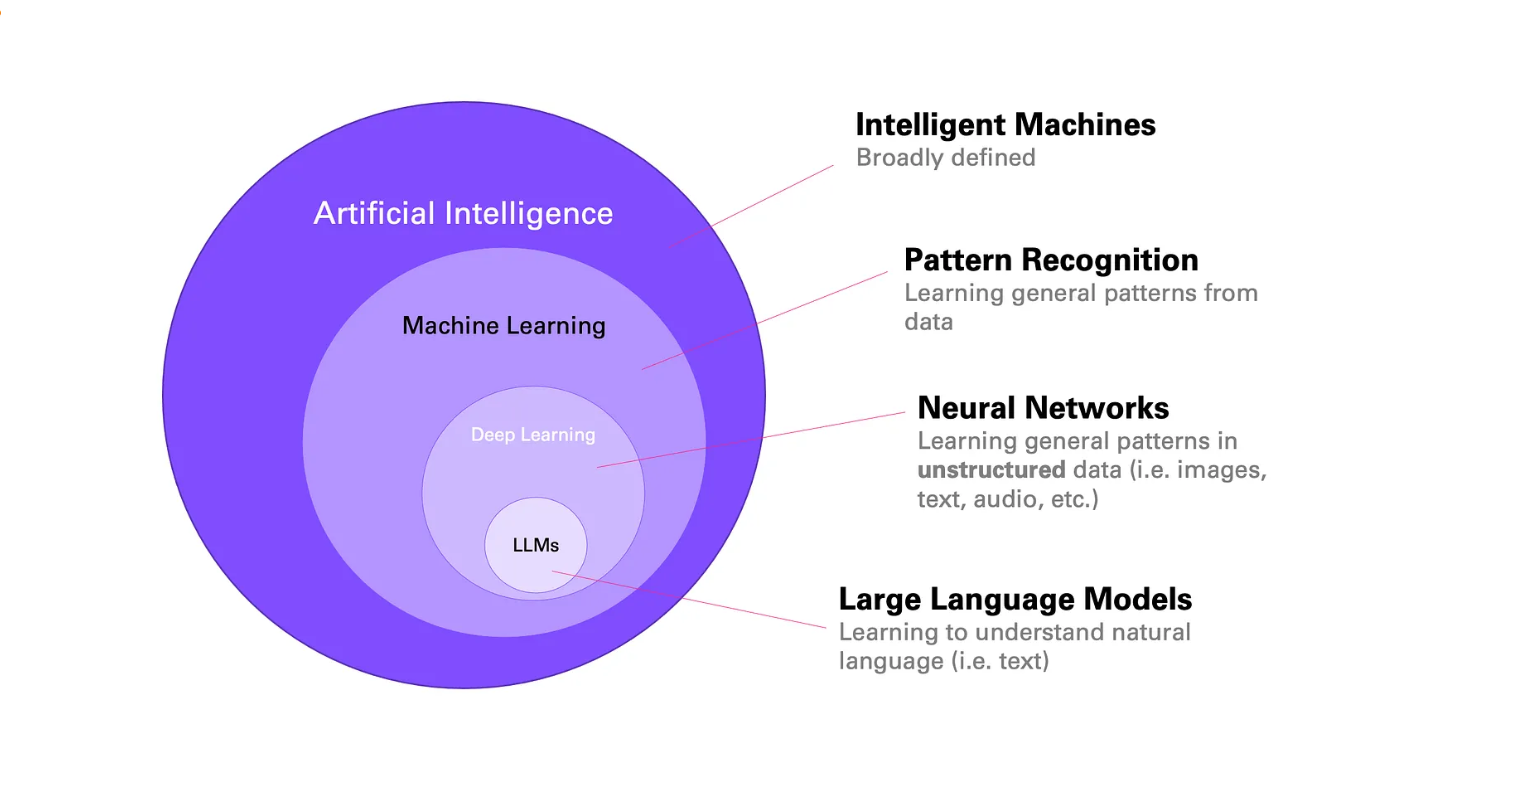
\includegraphics[width=0.83 \linewidth]{assets/art.png}
    \caption{The field of Artificial Intelligence in layers}
\end{figure}

\subsection{History}
%Through the 1990s and early 2000s, the AI industry was focused on small-scale applications and pipelines that were less computationally complex and time-intensive as shows the following figure 3.2 \cite{w10}. Let’s briefly look at the history of LLMs.
During the 1990s and early 2000s, the AI industry mostly worked on small projects that were not too complicated or time-consuming. This can be seen in \textbf{Figure \ref{fig:llm_historic}} \cite{w10}. Let's quickly talk about the history of LLMs.
\begin{figure}[H]
    \label{fig:llm_historic}
    \centering
    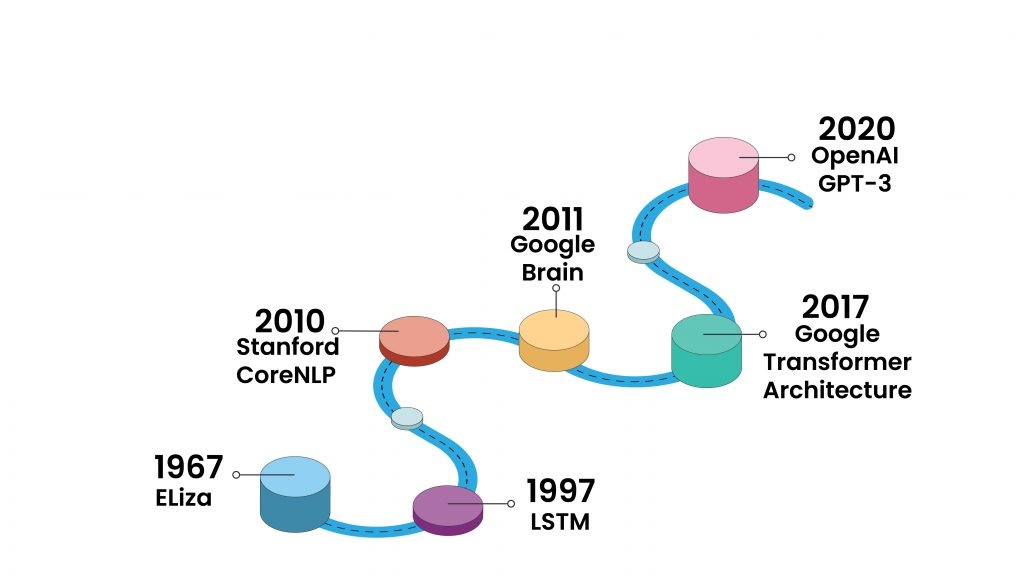
\includegraphics[width=1 \linewidth]{assets/llm_historic.jpeg}
    \caption{History of Large Language Models}
\end{figure}

When the ancients carefully recorded their knowledge on scrolls of papyrus and housed them in the legendary Library of Alexandria, they could not have even dreamed it possible that all that knowledge and more would be available at the fingertips of their descendants millenniums later. That’s the power and beauty of large language models. Not only can LLMs answer questions and solve complex problems, but they can also summarize huge volumes of work, as well as translate and derive context from various languages.
\vskip 0.5cm
The beginnings of big language models can be traced back to experiments with neural networks and neural information processing systems in the 1950s to help computers process and use natural language. Researchers at IBM and Georgetown University collaborated to develop a system that can translate phrases from Russian to English automatically. Research in machine translation started from there and gained a lot of recognition.
%The foundation of large language models can be traced back to experiments with neural networks and neural information processing systems that were conducted in the 1950s to allow computers to process natural language. Researchers at IBM and Georgetown University worked together to create a system that would be able to autoatically translate phrases from Russian to English. As a notable demonstration of machine translation, research in this field took off from there.
\vskip 0.5cm
The concept of LLMs started with Eliza, the first chatbot created by MIT researcher Joseph Weizenbaum in the 1960s. Eliza started the study of natural language processing NLP , laying the groundwork for advanced LLMs in the future. Then after about 30 years, in 1997, Long Short Term Memory LSTM networks were invented. Their arrival led to more advanced and sophisticated neural networks that could process larger amounts of data. Stanford's CoreNLP suite, launched in 2010, made it possible for developers to analyze feelings and identify entities in text.
%The idea of LLMs was first floated with the creation of Eliza in the 1960s: it was the world’s first chatbot, designed by MIT researcher Joseph Weizenbaum. Eliza marked the beginning of research into natural language processing (NLP), providing the foundation for future, more complex LLMs. Then almost 30+ years later, in 1997, Long Short-Term Memory (LSTM) networks came into existence. Their advent resulted in deeper and more complex neural networks that could handle greater amounts of data. Stanford’s CoreNLP suite, introduced in 2010, was the next stage of growth allowing developers to perform sentiment analysis and named entity recognition.
\vskip 0.5cm

In 2011, a smaller Google Brain with better features like word embeddings helped NLP systems understand context better. This was a big moment, with models becoming popular in 2017. Think, which is short for Generative Pre-trained Transformer, can create or "decode" new writing. Another example is BERT - Bidirectional Encoder Representations from Transformers. Wich analyze input text to make predictions or categorize it based on encoder parts.
%Subsequently, in 2011, a smaller version of Google Brain appeared with advanced features such as word embeddings, which enabled NLP systems to gain a clearer understanding of context. This was a significant turning point, with transformer models bursting onto the scene in 2017. Think GPT, which stands for Generative Pre-trained Transformer, has the ability to generate or “decode” new text. Another example is BERT – Bidirectional Encoder Representations from Transformers. BERT can predict or classify input text based on encoder components.
\vskip 0.5cm
%From 2018 onward, researchers focused on building increasingly larger models. It was in 2019 that researchers from Google introduced BERT, the two-directional, 340-million parameter model (the third largest model of its kind) that could determine context allowing it to adapt to various tasks. By pre-training BERT on a wide variety of unstructured data via self-supervised learning, the model was able to understand the relationships between words. In no time at all, BERT became the go-to tool for natural language processing tasks. In fact, it was BERT that was behind every English-based query administered via Google Search.
From 2018 onwards, researchers concentrated on creating bigger and bigger models. In 2019, Google researchers introduced BERT, a large model with 340 million parameters. It can understand context in both directions and can be used for different tasks. By training BERT on many different types of data without supervision, the model learned the relationships between words. BERT quickly became the top choice for tasks involving understanding and using human language. Actually, it was BERT that was responsible for every English query on Google Search.
\subsection{Types of Large Language Models (LLM)}
LLMs can be divided into three types pre-training models, fine-tuning models, and multimodal models. Different options have different benefits, depending on what you want to achieve:
%LLMs can be broken down into three types: pre-training models, fine-tuning models, and multimodal models. Each has its own advantage, depending on the goal:
\vskip 0.5cm
\begin{itemize}
    \item \textbf{Pre-training models}: are trained on huge quantities of data, which helps them comprehend a broad range of language patterns and constructs. A plus is that a pre-trained model tends to be grammatically correct!
    \item \textbf{Fine-tuning models}: are pre-trained on a large dataset and afterward are fine-tuned on a smaller dataset for a specific task (use case). They’re particularly good for sentiment analysis, answering questions, and classifying text.
    \item \textbf{Multimodal models}: combine text with other modes, such as images or video, to create more advanced language models. They can produce text descriptions of images and vice versa.
\end{itemize}

\subsection{Phases of training Large Language Models (LLMs)}
Large language models go through three main stages: pre training, fine-tuning for specific tasks, and learning from feedback from humans, as shown in \textbf{Figure \ref{fig:phases-llm}}\cite{w11}.
%Large language models undergo three main phases: pre-training, instruction fine-tuning, and reinforcement learning from human feedback as shows the following figure 3.3 \cite{w11}
\begin{figure}[H]
    \label{fig:phases-llm}
    \centering
    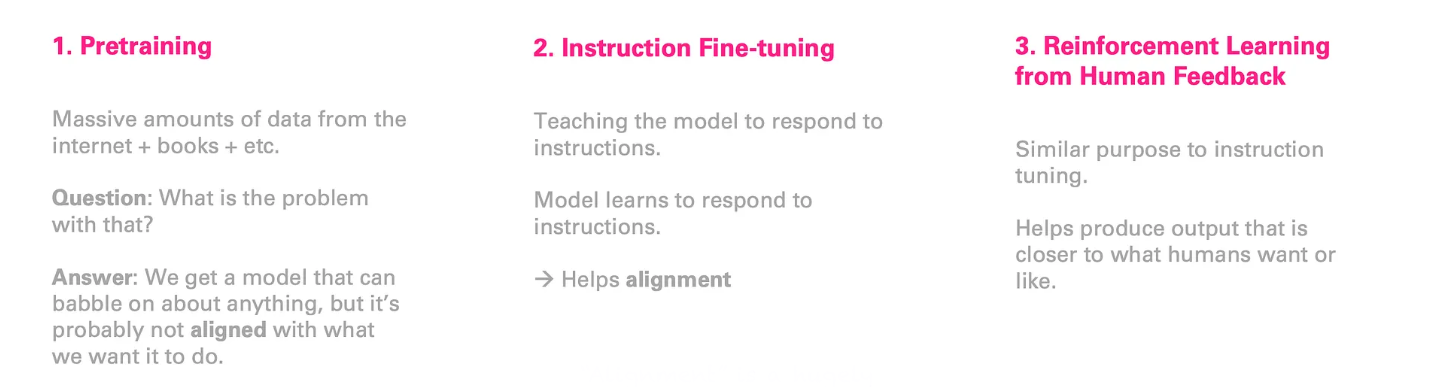
\includegraphics[width=0.9 \linewidth]{assets/gpt-phases.png}
    \caption{Phases of training LLMs}
\end{figure}

\subsubsection{Pre-training}
%stopped here !!!
This step needs a massive amount of data in order to train for predicting the next word. During this time, the model learns how to use language correctly and also gains knowledge about the world and develops new abilities.
%This stage requires massive amounts of data to learn to predict the next word. In that phase, the model learns not only to master the grammar and syntax of language, but it also acquires a great deal of knowledge about the world, and even some other emerging abilities
\vskip 0.5cm
%However, Pre-training a Large Language Model (LLM) primarily teaches it to ramble on about a topic, which can result in impressive output but poor performance in responding to specific inputs such as questions or instructions. This is because the LLM has not learned to be an assistant, but rather to complete input sequences. For example, when asked “What is your first name?”, a pre-trained LLM may respond with “What is your last name?” as it has been trained on many empty forms. The model struggles with following instructions because the structure of instruction followed by a response is not commonly seen in the training data. At this stage, the LLM is not aligned with human intentions, which is an important topic for LLMs. However, it can be taught to respond to instructions through further training. Despite initial difficulties, pre-trained LLMs are steerable, making it possible to teach them to follow instructions and align with human intentions.
However, training a large language model only teaches it to talk a lot about a topic, which can make it produce impressive results but not very good at answering specific questions or following instructions. The LLM has not learned to be an assistant, but instead to complete input sequences. For example, when someone asks "What is your first name?", a pre trained LLM might answer with "What is your last name?" because it has been trained on lots of empty forms. The model is having a hard time understanding instructions because it is not used to seeing a pattern where an instruction is given and then a response is expected. At this point, the LLM does not match up with what people want, which is a important concern for LLMs. However, it can learn to follow commands with more practice. Despite some challenges at first, pre-trained LLMs can be controlled and taught to follow directions and understand human goals.
\subsubsection{Instruction fine-tuning }
This is where instruction tuning comes in to adjust instructions. We use the pre-trained LLM with its current abilities and continue to predict one word at a time. This time, we only use high quality training data with instruction and response pairs.
%This is where instruction tuning comes in. We take the pre-trained LLM with its current abilities and do essentially what we did before — i.e., learn to predict one word at a time — but now we do this using only high-quality instruction and response pairs as our training data.
\vskip 0.5cm
%That way, the model un-learns to simply be a text completer and learns to become a helpful assistant that follows instructions and responds in a way that is aligned with the user’s intention. The size of this instruction dataset is typically a lot smaller than the pre-training set. This is because the high-quality instruction-response pairs are much more expensive to create as they are typically sourced from humans. This is very different from the inexpensive self-supervised labels we used in pre-training. This is why this stage is also called supervised instruction fine-tuning.
That way, the model un-learns to only complete sentences and learns to be a helpful assistant that follows directions and responds in a way that matches what the user wants. The size of this instruction dataset is usually much smaller than the pre-training set. high-quality instruction response pairs are very costly to make because they usually human annotated. This is very different from the cheap self-supervised labels we used in pre-training. This stage is also known as supervised instruction fine-tuning because of this reason.
%mdx
\subsubsection{Reinforcement Learning from Human Feedback (RLHF)}
At its core, RLHF uses human feedback to create a dataset of human preferences. This helps determine the reward function for a specific output. People can give feedback in many ways:
%On a basic level, RLHF implements human feedback to generate a human preferences dataset that ascertains the reward function for a desired outcome. Human feedback can be obtained in multiple ways:
\begin{itemize}
    \item \textbf{Order of preference}: People rank outputs in order of preference.
    \item \textbf{Demonstrations}: Humans write preferred answers to prompts.
    \item \textbf{Corrections}: Humans edit a model’s output to correct unfavorable behaviors.
    \item \textbf{Natural language input}: Humans provide descriptions or critiques of outputs in language. Once a reward model has been created, it’s used to train a baseline model with the help of reinforcement learning, which leverages the reward model to build a human values policy that the language model then uses to produce responses. ChatGPT is a good example of how a large language model uses RLHF to produce better, safer, and more engaging responses
    
\end{itemize}
%RLHF constitutes a major advancement in the realm of language models, providing a more controlled and reliable user experience. But there’s a tradeoff: RLHF introduces the biases of those who have contributed to the preference dataset used to train the reward model. So, while ChatGPT is geared toward helpful, honest, and safe answers, it’s still subject to the annotators’ interpretations of these answers. While RLHF improves consistency (which is great for the use of LLMs in search engines), it does so at the expense of creativity and diversity of ideas. There is still a lot to uncover in this area.
RLHF is a weighty step forward in language models, giving users a better and more reliable experience. However, there is a tradeoff, RLHF brings in the biases of the people who provided the data used to train the reward model. While ChatGPT aims to provide useful, honest, and self-confident answers, the way these answers are understood by the annotators can vary. RLHF improves consistency, but it reduces creativity and diversity of ideas. There is still a lot to discover in this area.
\subsection{Most Large Language Model Application}
%At first glance, LLMs can be used in any scenario where an organization needs to analyze, process, summarize, rewrite, edit, transcribe or extract insights from a dataset or input text. With adoption increasing, there are some practical applications of language models that appear to be promising.
At first look, LLMs can be used in any situation where a company needs to analyze, process,  summarize, rephrase, edit, transcribe or etract insights from a set of data or input text. With adoption increasing, there are some useful ways to use language models that seem to be very helpful.
\subsubsection{Translation With Language Models}
%One of the simplest practical applications for LLMs is to translate written texts. A user can enter text into a chatbot and ask it to translate into another language, and the solution will automatically begin translating the text.
One simple way to use LLMs is to change written words into a different language. A person can type in words to a chatbot and ask it to change them to a different language, and the chatbot will start translating the words automatically.
\subsubsection{Content Creation}
Another very common use for language models is creating content. LLMS allows people to create many different types of written content, like blogs, articles, short stories, summaries, scripts, questionnaires, surveys, and social media posts. The quality of these outputs relies on the provided in the initial prompt.
%Another increasingly common use case for language models is content creation. LLMS enables users to generate a range of written content from blogs and articles to short stories, summaries, scripts, questionnaires, surveys, and social media posts. The quality of these outputs depends on the details provided in the initial prompt.
\vskip 0.5cm
%If LLMs aren’t used to generate content directly, they can also be used to help with ideation. According to Hubspot, 33\% of marketers who use AI use it to generate ideas or inspiration for marketing content. The main value here, is that AI can speed up the content generation process. It’s worth noting that there are also tools like DALL-E, MidJourney, and Stable Diffusion that allow users to generate images based on a written prompt.
If LLMs are not used to create content, they can still be used to come up with new ideas. According to Hubspot, 33\% of marketers who use AI use it to come up with ideas or inspiration for marketing content. The key benefit here is that AI can make the process of creating content faster. There are tools like DALL E, MidJourney, and Stable Diffusion that let you make pictures from written prompts.
\subsubsection{Search}
Many users will first have experimented with generative AI as an alternative search tool. Users can ask a chatbot questions in natural language and will receive an instant response with insights and facts on potentially any topic.
\vskip 0.5cm
Using tools like Bard or ChatGPT to search for information gives you access to a lot of different information, but not all of it may be correct. 
%While using solutions like Bard or ChatGPT as a search tool provides access to a wide-range of information, it’s important to be aware that not all of this content is accurate.
\vskip 0.5cm
%Language models are prone to hallucination, and have a tendency to invent facts and figures. For this reason, it’s a good idea for users to double-check any factual information presented by LLMs so they can avoid being misled by misinformation.
Language models often make mistakes and can come up with false information. It is important for users to verify any facts shared by LLMs to avoid being misled by misinformation.
\subsubsection{Detecting and Preventing Cyber Attacks}
Another interesting use of language models in cybersecurity is identifying cyberattacks. LLMs are able to analyze big sets of data from a company's network and can detect patterns that show a harmful cyber attack and send a warning.
%Another interesting cybersecurity use case for language models is detecting cyberattacks. This is because LLMs have the ability to process large data sets collected throughout an enterprise network and can spot patterns that indicate a malicious cyber attack and generate an alert.
\vskip 0.5cm
So far, some companies are testing new technology to find and stop cybersecurity threats. For instance, earlier this year SentinelOne introduced a solution driven by LLM that can automatically search for threats and start automated responses of malicious activity.
%So far a number of cybersecurity vendors have begun experimenting with the technology for threat detection. For example, early this year SentinelOne released an LLM-driven solution that can automatically hunt for threats and initiate automated responses to malicious activity.
\vskip 0.5cm
%Another approach demonstrated by Microsoft Security Copilot, allows users to scan their environments for known vulnerabilities and exploits, and can generate reports on potential security events in minutes to equip human defenders to respond.
Another way shown by Microsoft Security Copilot, lets users check their systems for known weaknesses and attacks, and can create reports about possible security issues in a few minutes so that people can react quickly.
\subsubsection{Code Development}
Generative AI tools can create both natural language and code in languages like JavaScript, Python, PHP, Java, and C\#.
%Generative AI tools not only have the ability to generate natural language, but can generate code in languages like JavaScript, Python, PHP, Java, and C\#.
\vskip 0.5cm
\textsc{The language models can help non-technical users  to create simple code. Can write basic code for simple projects, but has difficulties with larger and more complex tasks  that are bigger in scope and scale.}
\vskip 0.5cm
%Thus programmers should double-check code for functionality and security issues during development to avoid disruption post-deployment. They can also be used to help debug existing code or even generate accompanying documentation so that users don’t have to spend time doing it manually.
Programmers need to carefully review their code for any problems with how it works or how secure it is before they finish working on it. This will help prevent any issues from happening after the code is in use. They can also be used to help fix problems in code or create documentation automatically, saving users time.
\subsection{Large Language Model tools}
large language models like LlaMA have various versions, such as llama2 7b, llama2 13b, and llama2 70b. These versions reflect the model’s size and capacity, with larger models having more parameters and being able to handle more complex tasks. The purpose of versioning is to offer different sizes and capabilities of the model to fit different needs and uses. For instance, a small model like llama2 7b could work well for a chatbot, while a larger model like llama2 70b might be better for generating content. Versioning allows developers to pick the best model for their needs, balancing resources and requirements.
%Large language models, such as LlaMA, have different versions, including llama2-7b, llama2-13b, and llama2-70b. These versions reflect the model’s size and capacity, with larger models having more parameters and being able to handle more complex tasks. The goal of versioning is to provide different sizes and capacities of the model to suit various applications and use cases. For example, a smaller model like llama2-7b may be suitable for a chatbot application, while a larger model like llama2-70b may be more appropriate for a content generation task. Versioning allows developers to choose the best model for their specific needs, balancing computational resources and task requirements.
\subsubsection{Open-source LLM Models}


\begin{longtable}{|>{\centering\arraybackslash}p{2.5cm}|>{\centering\arraybackslash}p{2cm}|>{\centering\arraybackslash}p{4cm}|>{\centering\arraybackslash}p{2.5cm}|>{\centering\arraybackslash}p{2.5cm}|}
    \caption{Overview of Various Language Models} \label{tab:models} \\
    \hline
    \rowcolor[gray]{0.8}
    \textbf{Model} & \textbf{Developer} & \textbf{Key Features} & \textbf{Theoretical Context Window} & \textbf{Application} \\
    \endfirsthead
    
    \hline
    \rowcolor[gray]{0.8}
    \textbf{Model} & \textbf{Developer} & \textbf{Key Features} & \textbf{Theoretical Context Window} & \textbf{Application} \\
    \endhead
    
    \hline
    \multicolumn{5}{|r|}{{Continued on next page}} \\
    \endfoot
    
    \hline
    \endlastfoot
    
    LlaMA 2 & Meta AI & Ranges from 7 billion to 70 billion parameters, designed for reasoning, coding, proficiency, and knowledge tests. & 4096 tokens & Reasoning, coding, proficiency tests \\
    \hline
    BLOOM & BigScience & A multilingual LLM with 176 billion parameters, covering 46 natural and 13 programming languages. & 2048 tokens & Multilingual understanding, translation \\
    \hline
    BERT & Google & A transformer-based model focusing on bidirectional training, with a deep understanding of language context. & 512 tokens & Natural language understanding, context analysis \\
    \hline
    OPT-175B & Meta AI Research & A model with 175 billion parameters, designed for zero- and few-shot learning, boasting a low carbon footprint for its training. & 2048 tokens & Zero-shot learning, efficient training \\
    \hline
    Xgen-7B & Salesforce & Excels in processing up to 8,000 tokens, suitable for detailed conversations and comprehensive summarization. & 8000 tokens & Conversations, summarization \\
    \hline
    Falcon-180B & Technology Innovation Institute & A causal decoder-only model with 180 billion parameters, supporting multiple languages and excelling in various tasks. & 2048 tokens & Language tasks, multilingual support \\
    \hline
    Mistral 7B & Mistral AI & A model with 7.3 billion parameters, optimized for English language tasks and coding, efficient in resource usage. & 4096 tokens & English tasks, coding \\
    \hline
    CodeGen & Not specified & Focused on program synthesis across multiple languages, transforming English prompts into executable code. & 2048 tokens & Program synthesis, code generation \\
    \hline
    Mixtral 8x7B & Mistral AI & An enhanced version of Mistral with improved performance and efficiency for a broader range of applications. & 4096 tokens & Broad applications, enhanced performance \\
    \hline
    \end{longtable}
    




\section{Technologies and Models Choice}
\subsection{Comparison Table: LlamaIndex vs LangChain}
LlamaIndex is made for creating search and retrieval application, as shown in \textbf{Table \ref{tab:FC}}. It helps you search for information and find the right documents easily using LLMs. LlamaIndex is the best choice for projects that focus on making a search and retrieval application , efficient,  prioritizing efficiency and simplicity while concentrating on specific tasks. Our project aims to create an application that can work well with different software, is easily adjustable, and can grow as needed. Langchain is a great option for this. Nevertheless, each option is unique in how it works and what it's meant for, making sure it's a perfect fit for our particular requirements.
%LlamaIndex is specifically designed for building search and retrieval application, as displays the following table 3.2. It provides a simple interface for querying LLMs and retrieving relevant documents. Llama Index emerges as the preferred option for project revolves around the development of a streamlined search and retrieval application, prioritizing efficiency and simplicity while concentrating on specific tasks.Otherwise, our project is a process of constructing a versatile application flexible(seamless integration with various software), scalable and aiming for adaptability, Langchain and  makes for an excellent choice. Neverthelss, Each choice is distinct in its approach and purpose, ensuring a tailored fit for our specific needs.
\vskip 0.5cm
%However, LangChain’s robust ecosystem provides extensive resources and support, making it an ideal platform for developing advanced chatbots. In fact, LlamaIndex is built on top of LangChain underscores the latter’s versatility and critical role in the language model development landscape. This, combined with the direct integration with LangSmith, ensures that LangChain offers a comprehensive solution for creating chatbots capable of delivering high-quality, contextually relevant responses.
LangChain's robust ecosystem offers a lot of help and resources, making it a great place to create advanced chatbots. In fact, LlamaIndex is based on LangChain, which shows how important it is in developing language models. This, along with the direct connection to LangSmith, makes sure that LangChain provides a complete solution for making chatbots that can give top-quality, contuextually relevant responses.
\begin{table}[H]
\label{tab:FC}
\begin{center}
\caption{Feature Comparison: LlamaIndex vs. LangChain}
\begin{tabular}{|l|p{5cm}|p{5cm}|}
\hline
 \rowcolor[gray]{0.8} \textbf{Feature/Aspect} & \textbf{LlamaIndex} & \textbf{LangChain} \\
\hline
\textbf{Overview} & A tool for efficient information indexing and retrieval, used with AI models for enhanced retrieval. & A framework for building language models, focusing on easy integration with external knowledge sources like RAG. \\
\hline
\textbf{Pros} & - Efficient indexing and retrieval \newline - Scalable for large datasets \newline - Integrates with various AI models & - Designed for language applications \newline - Easy integration with tools like LangSmith \newline - Supports RAG \newline - Active community and updates \\
\hline
\textbf{Cons} & - Focused on indexing; additional tools needed for chatbots \newline - More setup for language tool integration & - More complex initial setup \newline - Requires familiarity with its ecosystem \\
\hline
\end{tabular}
\end{center}
\end{table} 



\subsection{Comparison of Open-Source LLM Models}
The decision between Mistral and Mixtral models depends on the type of equipment you have and what the project requires. Mixtral 8x7B is great for NLP tasks that need a lot of parameters. It works well even when you have limited resources, like in \textbf{Table \ref{tab:model_specs}}. It performs really well. On the other hand, Mistral 0.2V 7B is a good choice for projects with standard hardware capabilities. It gives a good balance between performance and efficiency.
%The choice between Mistral and Mixtral models depends on the specific hardware available and the project's needs. Mixtral 8x7B, with its high parameter count, is ideal for demanding NLP tasks where computational resources are not a constraint, as shown in the following table 3.3, offering superior performance. On the other hand, Mistral 0.2V 7B provides a balanced option for projects with moderate hardware capabilities, offering a good trade-off between performance and efficiency.
\begin{table}[H]
\begin{center}
\caption{open-source llm model Specifications}
\label{tab:model_specs}
\begin{tabular}{|c|c|p{2cm}|p{2cm}|p{2cm}|p{2cm}|}
\hline
\rowcolor[gray]{0.8} 
\textbf{Model} & \textbf{Parameters} & \textbf{Hardware Requirements} & \textbf{Performance} & \textbf{Use Cases} & \textbf{Context Window} \\ \hline
Mixtral 8x7B & 56B & High & Very high accuracy & Demanding NLP tasks & Large \\ \hline
Mistral 0.2V 7B & 7B & Moderate & Balanced performance & General NLP tasks & Moderate \\ \hline
Llama2 13B & 13B & Moderate to High & High performance & Detailed language understanding & Moderate to Large \\ \hline
Llama2 7B & 7B & Low to Moderate & Solid performance & Development and testing & Moderate \\ \hline
\end{tabular}
\end{center}
\end{table}
\subsection{Performance Benchmarking of common Language Models}
Table 3.4 \cite{w12} shows how different language models perform on different tests. These models come in different designs and sizes. They are tested on various benchmarks to see how well they can do tasks like reading, reasoning, and understanding language.
%The following table 3.4 \cite{w12} presents a comprehensive comparison of the performance of various language models across multiple benchmark datasets. These models encompass a range of architectures and sizes, each evaluated on key benchmarks that assess their proficiency in diverse linguistic tasks such as reading comprehension, commonsense reasoning, and language understanding. 
\vskip 0.5cm
The performance metrics include Average Score, ARC AI2 Reasoning Challenge , HellaSwag, MMLU Mean Multi Labeling Unweighted , TruthfulQA, Winograd Schema Challenge Winogrande , and GSM8K General Language Understanding Evaluation Benchmark . The \textbf{Table \ref{tab:MC}} focuses on showing the strengths and weaknesses of various language models when it comes to understand different types of natural language tasks.
%The performance metrics include Average Score, ARC (AI2 Reasoning Challenge), HellaSwag, MMLU (Mean Multi-Labeling Unweighted), TruthfulQA, Winograd Schema Challenge (Winogrande), and GSM8K (General Language Understanding Evaluation Benchmark). The table aims to provide insights into the relative strengths and weaknesses of different language models in addressing a wide spectrum of natural language understanding tasks.

\begin{table}[H]
    \centering
    \caption{Model Comparison}
    \label{tab:MC}
    \begin{tabular}{|>{\raggedright\arraybackslash}p{2.5cm}|c|c|c|c|>{\raggedright\arraybackslash}p{2cm}|>{\raggedright\arraybackslash}p{2cm}|c|}
    \hline
    \rowcolor[gray]{0.8} 
    \textbf{Model} & \textbf{Average} & \textbf{ARC} & \textbf{HellaSwag} & \textbf{MMLU} & \textbf{TruthfulQA} & \textbf{Winogrande} & \textbf{GSM8K} \\
    \hline
    mistralai/Mix-tral-8x7B-Instruct-v0.1 & 72.62 & 70.22 & 87.63 & 84.88 & 71.16 & 64.58 & 81.37 \\
    \hline
    meta-llama/Llama-2-70b-hf & 67.87 & 67.32 & 87.33 & 83.74 & 69.83 & 44.92 & 54.06 \\
    \hline
    tiiuae/falcon-40b & 58.07 & 61.86 & 85.28 & 81.29 & 56.89 & 41.65 & 21.46 \\
    \hline
    mistralai/Mis-tral-7B-Instruct-v0.2 & 65.71 & 63.14 & 84.88 & 77.19 & 60.78 & 68.26 & 40.03 \\
    \hline
    meta-llama/Llama-2-13b-hf & 55.69 & 59.39 & 82.13 & 76.64 & 55.77 & 37.38 & 76.64 \\
    \hline
    meta-llama/Llama-2-7b-hf & 50.97 & 53.07 & 78.59 & 74.03 & 46.87 & 38.76 & 14.48 \\
    \hline
    tiiuae/falcon-7b & 44.17 & 47.87 & 78.13 & 72.38 & 27.79 & 34.26 & 4.62 \\
    \hline
    Salesforce/cod-egen-16B-nl & 42.59 & 46.76 & 71.87 & 32.35 & 33.95 & 67.96 & 2.65 \\
    \hline
    Salesforce/cod-egen-6B-nl & 40.00 & 42.32 & 68.59 & 25.93 & 34.47 & 66.46 & 2.20 \\
    \hline
    Salesforce/cod-egen-6B-multi & 32.43 & 27.22 & 41.11 & 25.71 & 45.65 & 53.91 & 0.99 \\
    \hline
    \end{tabular}
    \end{table}


\subsection{Comparison of Embedding Models}
%Considering the efficiency, performance, and particularly the large context window provided by the Nomic Embedding Model,as shown the following tbale 3.4, it is our chosen model for embedding. This decision is based on its ability to handle complex NLP tasks requiring deep contextual understanding. The model's scalability with hardware ensures it meets our diverse application needs, making it the optimal choice despite varying hardware requirements.
We have chosen the BGE Embedding Model as our preferred model for embedding because it offers high efficiency, performance, and a large context window, as shown in \textbf{Table \ref{tab:EMS}}. This choice is made because
can handle difficult NLP tasks that need a deep understanding of context. The model's ability to work well with different types of hardware helps it meet many needs for different applications, which is why it's the best choice even with different hardware requirements.
\begin{table}[H]
\label{tab:EMS}
\begin{center}
\caption{Embedding Models Specifications}

\begin{tabular}{|p{2cm}|c|c|p{2.5cm}|p{2cm}|p{2cm}|p{2.2cm}|}
\hline
\rowcolor[gray]{0.8} 
\textbf{Model} & \textbf{Parameters} & \textbf{Efficiency} & \textbf{Performance} & \textbf{Use Cases} & \textbf{Context Window} & \textbf{Hardware Requirements} \\ \hline
Ada002 & Small & High & Quick, lightweight tasks & General NLP tasks & Small & Low-end GPUs/CPUs \\ \hline
BERT-base & 110M & Moderate & Solid performance for a variety of tasks & Wide range of NLP tasks & 512 tokens & Consumer-grade GPUs \\ \hline
GPT-2 & 1.5B & Low & High-quality text generation & Text generation, conversation & 1024 tokens & High-end GPUs \\ \hline
Nomic Embedding Model & Varies & Varies & Exceptional across tasks & Large context window tasks & 8194 tokens & Varies; scalable to hardware \\ \hline
\end{tabular}
\end{center}
\end{table}

\subsection{Retrieval Augmented Generation (RAG)}
RAG (Retrieval-Augmented Generation) empowers LLMs by fetching relevant information from external knowledge bases, enhancing their responses with factual grounding as shows the following \textbf{Figure \ref{fig:RAG}}\cite{w13}.
\begin{figure}[H]
    \label{fig:RAG}
    \centering
        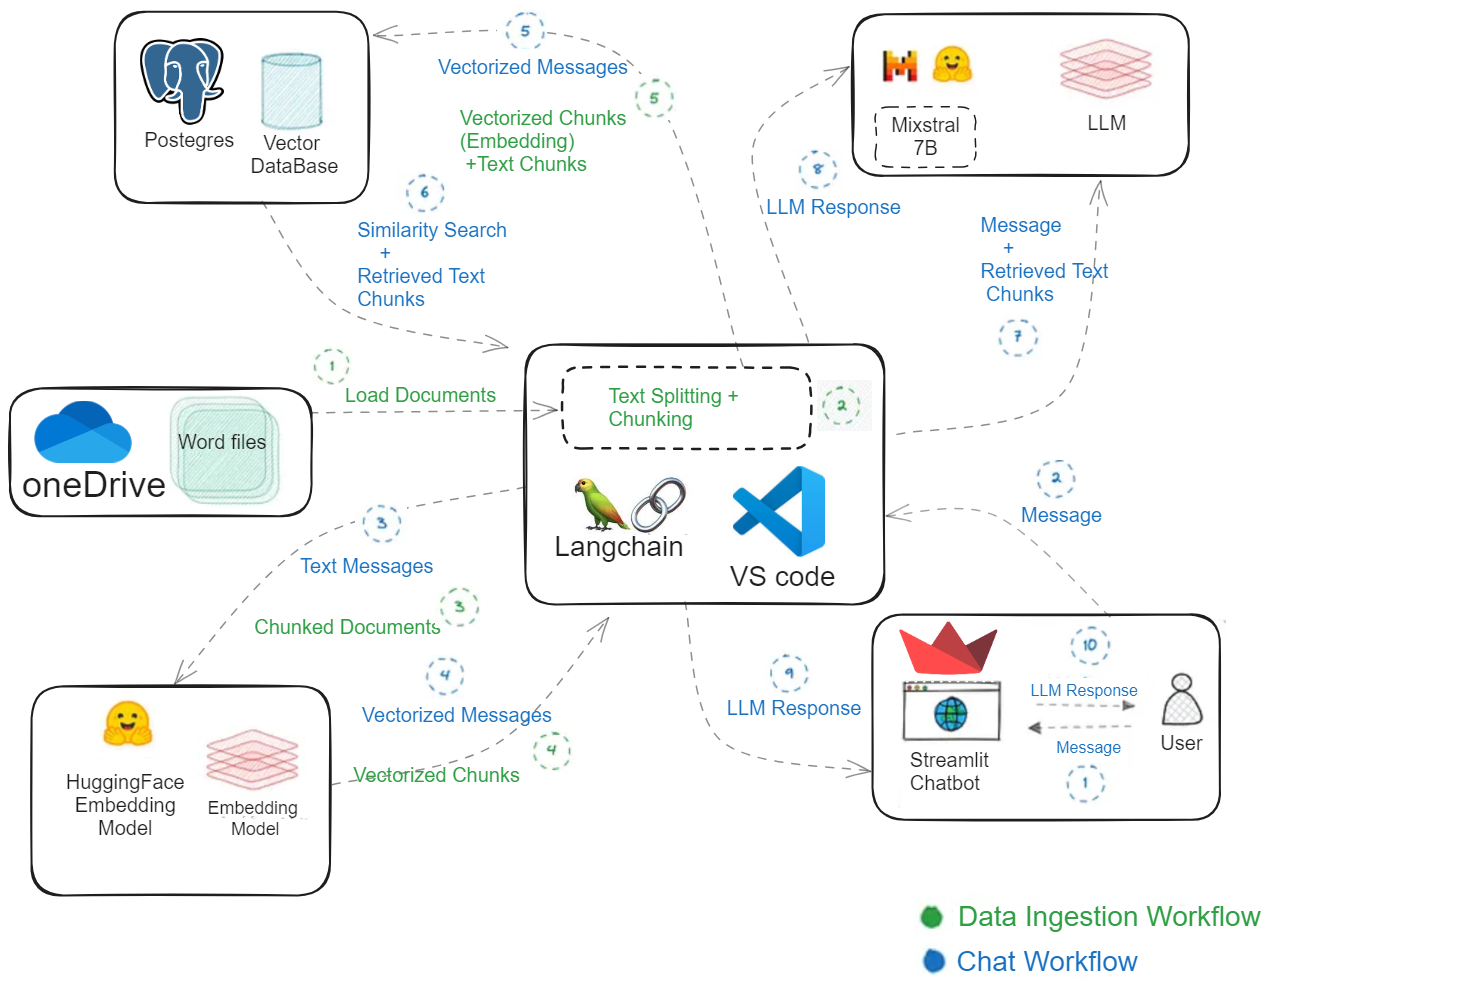
\includegraphics[width=1 \linewidth]{assets/pipeline_rag.png}
    \caption{RAG pipeline}
\end{figure}
The process begins with loading a huge data base or corpus containing relevant information . This information base might contain of content from diverse sources such as books, articles, websites, or any other organized or unstructured data stores.
\vskip 0.5cm
Once the data base is loaded , it s divided into reasonable chunks or sections to encourage effective recuperation . Chunking guarantees that the retrieval process is versatile and doesn t overload the framework with excessive data at once.
\vskip 0.5cm
Each chunk of information is at that point encoded into a numerical representation, ordinarily utilizing methods like word embeddings or more progressed methods such as transformer based models like BERT (Bidirectional Encoder Representations from Transformers) . This vectorization process converts the literary data into high-dimensional vectors that capture semantic and relevant connections between words and expressions.
\vskip 0.5cm
when a query is received , it's also vectorized utilizing the same encoding method as the information base. This grants for effective closeness computation between the query vector and the vectors representing chunks of information inside the information base.
\vskip 0.5cm
Retrieval procedures like approximate nearest neighbor search or other similarity based methods are then employed to recognize the foremost significant chunks of information that match the query vector. chunks of information are recuperated , they are concatenated to make the setting or background data for the discussion . This setting gives the fundamental foundation for creating coherent and pertinent responses.
\vskip 0.5cm
The concatenated context, along with the primary query , serves as input to a large language model such as GPT Generative Pre-trained Transformer or a comparative architecture .
\vskip 0.5cm
large language model creates responses based on the input context and query . By leveraging the pertinent information recovered from the vectorestore. However, the responses are not only fluent and coherent but also grounded in retrieved context.
\vskip 0.5cm
The last response , created by the language model is then displayed to the client or coordinates into the conversational interface.
\vskip 0.5cm
at the end of the process, the generated response is displayed to the client or integrated into the conversational interface. In general, the Rag system consistently integrates the processes of data recovery and generation to create contextually pertinent and coherent responses in conversational applications.
% \begin{itemize}
%     \item \textbf{Message}: The process begins with the user posing a question. This question is the input that needs to be addressed or answered. wich then chunked into vectorized chunks.
%     \item \textbf{Streamlit Chatbot}: This component serves as the essential interface for client interaction with the chatbot. Clients can input their queries here, which the chatbot at that point forms to create and show smart responses . This interaction encourages a consistent communication stream between the client and the chatbot, improving the overall user experience.
%     \item \textbf{Vectorized Chunks}: This term refers to segments of text extracted from a larger corpus that have been converted into embeddings. These embeddings are numerical representations that encapsulate the semantic essence of the text. This transformation enables more efficient and accurate methods for comparing and retrieving information based on content similarity. These are specific segments of text chosen from the corpus by the  Retriever, identified as relevant to the user s message . Their relevance is assessed through the semantic similarity between the embeddings of the user's question and those of the text stored within the vector database. This process ensures that the most pertinent data is retrieved to accurately address the user's needs.
%     \item \textbf{Documents}: These are crucial components within the Rag Retrieval Augmented Generation pipeline. Sourced from various storage solutions like OneDrive or local hardware devices , these documents form the basis for extracting pertinent data . This data is then utilized to make accurate reactions to user inquiries , ensuring that the generated answers are both important and informed.
%     %\item \textbf{Prompt Template}: The relevant chunks and the user question are combined into a prompt template. This template is structured in a way that makes it understandable and usable for a Large Language Model (LLM), preparing it for the query phase.
%     \item \textbf{LLM Query}: The structured prompt is then sent as a query to a Large Language Model. Various LLMs, like those provided by Hugging Face, Cohere, or OpenAI, can be used. This step involves the generative model considering the information from the prompt to generate an accurate and informed response.
%     \item \textbf{LLM Response}: Finally, the Large Language Model generates an answer to the user's question, drawing from the information provided in the prompt and its pre-trained knowledge.
% \end{itemize}


\section{RAG Applications}
Retrieval-augmented generation models have demonstrated versatility across multiple domains. Some of the real-world applications of RAG models are :
\vskip 0.5cm
\begin{itemize}
    \item  \textbf{Advanced question-answering systems}:RAG models can power question-answering systems that retrieve and generate accurate responses, enhancing information accessibility for individuals and organizations. 
    \item \textbf{Content creation and summarization}: RAG models not only streamline content creation by retrieving relevant information from diverse sources, facilitating the development of high-quality articles, reports, and summaries, but they also excel in generating coherent text based on specific prompts or topics.
    \item \textbf{Conversational agents and chatbots}:RAG models enhance conversational agents, allowing them to fetch contextually relevant information from external sources. This capability ensures that customer service chatbots, virtual assistants, as well as other conversational interfaces deliver accurate and informative responses during interactions. Ultimately, it makes these AI systems more effective in assisting users.
    \item \textbf{Information retrieval}:RAG models enhance information retrieval systems by improving the relevance and accuracy of search results.
\end{itemize}
%https://www.google.com/url?sa=t&rct=j&q=&esrc=s&source=web&cd=&cad=rja&uact=8&ved=2ahUKEwidqtXYhoSFAxW6hf0HHRBzDucQFnoECBwQAQ&url=https%3A%2F%2Fhyperight.com%2F7-practical-applications-of-rag-models-and-their-impact-on-society%2F&usg=AOvVaw2zoZR6i6LGVF1jSKhZmGGX&opi=89978449

\section{Conclusion}
%In conclusion, this chapter has offered a comprehensive definition of llm and overview of historical AI story, discussing the common llm types, phases of training and application.Additionally, various LLM tools have been presented, highlighting the usefulness of Langchain over LlamaIndex, as well as existing competing language and embedding models. Finally, this chapter have included the RAG pipeline of our chatbot and its main application.
In conclusion, this chapter has provided a detailed explanation of LLM and a summary of the history of AI. It talks about different types of LLM, how they are trained, and where they are used. It also introduces various tools for LLM and compares Langchain with LlamaIndex, discusses other competing language and embedding models. Finally, this chapter has included the RAG pipeline of our chatbot and its main application.
\vskip 0.5cm
In the next chapter, we will present the chatbot process of the augmented search generation in detail.



